\documentclass{article}
\usepackage[utf8]{inputenc}
\usepackage{graphicx}

\title{Project Report}
\author{Hieu Mai }
\date{November 2020}

\begin{document}

\maketitle
\label{intro}
This document explains about the creating virtualized network with data center topology and DDos attack on it. Project is done on Ubuntu 18. Mininet and python were installed as prerequisite.
\section{Part A – Python code for data center network topology}
\label{}
For this topology, I used OVSKernelSwitch type 20 switches, 16 host with predefined Ips, added links between switches and hosts. I also added specific Ips for the switches. I install and ran the python code from terminal window. I called the dump command to see the connection details. 

\begin{figure}[ht]
\centerline{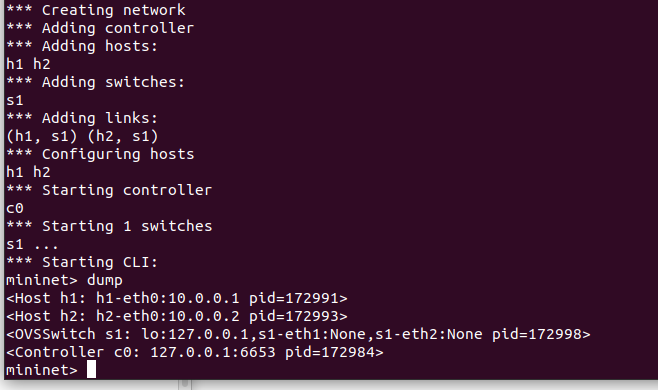
\includegraphics[scale=0.8]{parta.PNG}}
\caption{Start of mininet application}
\label{fig}
\end{figure}

\section{Part B - DDos attack}
\label{}
Installed Scapy by using following command:

sudo pip3 install scapy

I ran the code and entered source/system IP, target/host IP (I chose 10.0.0.1 Ip for DDos attack), I used both port as 80. I got permission error. I ran the code in sudo, it worked and start sending packets from source to target.

\begin{figure}[ht]
\centerline{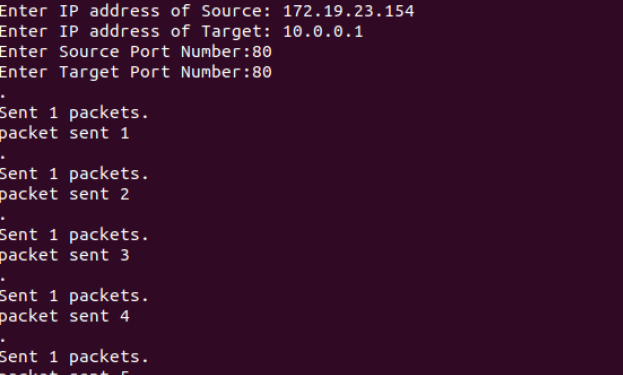
\includegraphics[scale=0.8]{partb.PNG}}
\caption{DDoS attack}
\label{fig}
\end{figure}

\section{Part C - Multiple Host DDos attack}
\label{1}
I modified my code for part B and used it for configuration multiple sources. I added ‘cpu=f’ while adding all hosts and ‘bw=10’ while adding all links as asked in the assignment. 

For single targeted host, it is observed that the data center topology with no bandwidth host limitation’s network was full and not recovering.

\begin{figure}[h]
\centerline{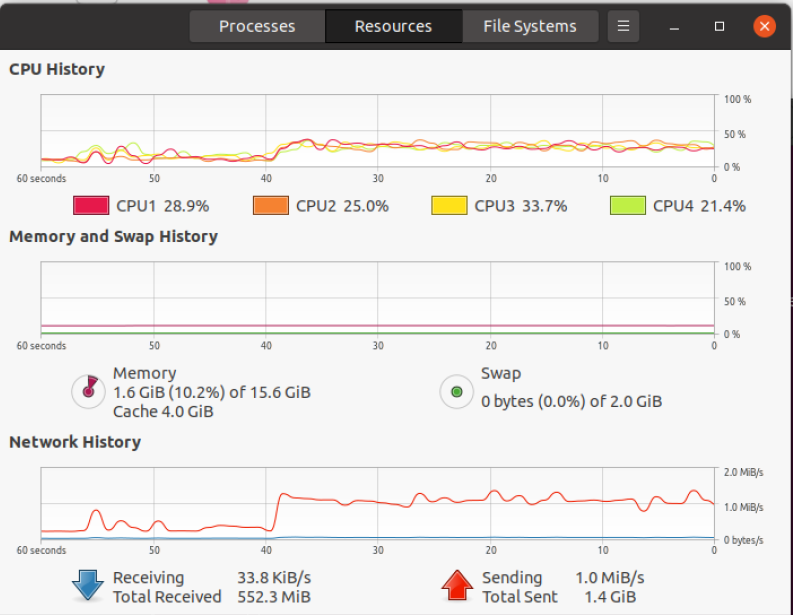
\includegraphics[scale=0.5]{DDOSperformance2.PNG}}
\caption{Without limit network}
\label{fig}
\end{figure}

\label{2}
While the data center topology with cpu and bandwidth limitation was not exceeding a certain amount of network.

\begin{figure}[h]
\centerline{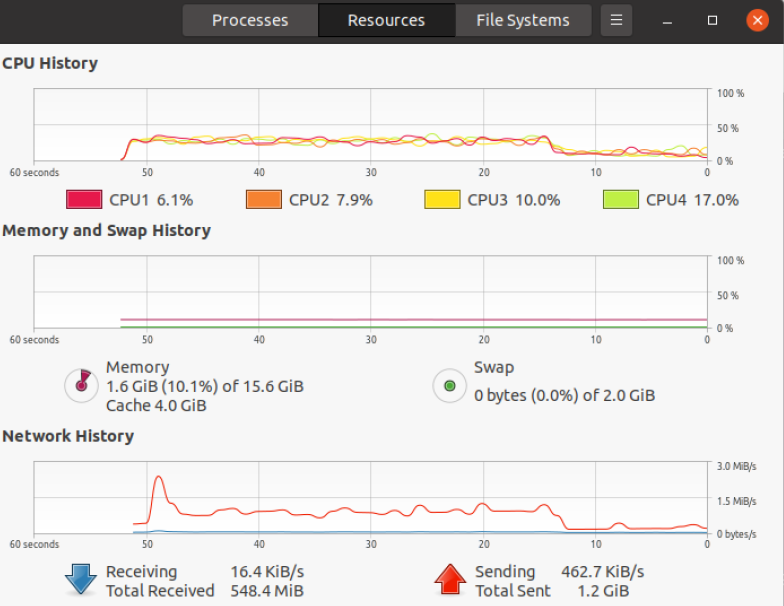
\includegraphics[scale=0.5]{DDOSperformance1.PNG}}
\caption{With limit network}
\label{fig}
\end{figure}

\end{document}
